%\begin{wrapfigure}[0]{r}[0cm]{3cm}
% \vspace{-6cm}
% 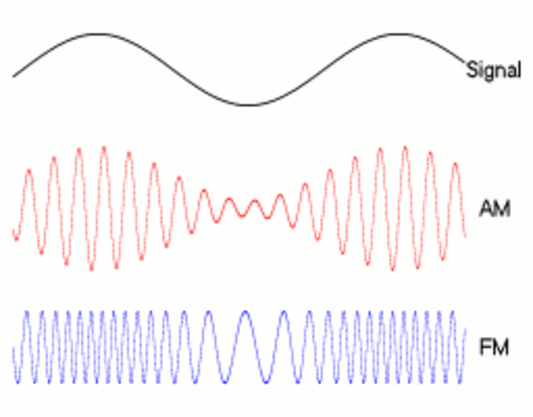
\includegraphics[scale=0.4]{Frequenzaufbereitung/Bilder/Amfm3-en-de.pdf}
% \vspace{-6cm}
%\end{wrapfigure}

\section*{Theorie- und Prüfungsfragen} 

\mucho{1}{TK105}
{In einem NF-Verstärker erfolgt die unerwünschte Gleichrichtung eines HF-Signals wahrscheinlich}%Frage
{an der Lautsprecherleitung.}%A
{an einem Basis-Emitter-Übergang.}%B
{an der Verbindung zweier Widerstände.}%C
{an einem Kupferdraht.}%D
{B}%Lösung

\mucho{2}{TK301}
{Um die Störwahrscheinlichkeit zu verringern, sollte die benutzte Sendeleistung}%Frage
{nur auf den zulässigen Pegel eingestellt werden.}%A
{auf das für eine zufrieden stellende Kommunikation erforderliche Minimum eingestellt werden.}%B
{auf die für eine zufrieden stellende Kommunikation erforderlichen 750 W eingestellt werden.}%C
{die Hälfte des maximal zulässigen Pegels betragen.}%D
{B}%Lösung

\mucho{3}{TK302}
{Wie kann man hochfrequente Störungen reduzieren, die durch Harmonische hervorgerufen werden? Sie können reduziert werden durch ein ...}%Frage
{Hochpassfilter}%A
{ZF-Filter}%B
{Nachbarkanalfilter}%C
{Oberwellenfilter}%D
{D}%Lösung

\mucho{4}{TK112}
{Ein Fernsehgerät wird durch das Nutzsignal einer KW-Amateurfunkstelle gestört. Wie kann das Signal in das Fernsehgerät eindringen?}%Frage
{Über jeden beliebigen Leitungsanschluss
und/oder über die ZF-Stufen.}%A
{Über die Antennenleitung und über alle größeren ungeschirmten Spulen im Fernsehgerät (z.B. Entmagnetisierungsschleife).}%B
{Über die Stromversorgung des Senders und die Stromversorgung des Fernsehgeräts.}%C
{Über die Fernsehantenne bzw. das Antennenkabel sowie über die Bildröhre.}%D
{A}%Lösung

\mucho{5}{TK306}
{Welches Filter sollte im Störungsfall vor die einzelnen Leitungsanschlüsse eines UKW- oder Fernsehrundfunkgeräts oder angeschlossener Geräte eingeschleift werden, um Kurzwellensignale zu dämpfen?}%Frage
{Ein Bandpassfilter bei 30 MHz unmittelbar vor dem Antennenanschluss und ein Tiefpassfilter in das Netzkabel der gestörten Geräte.}%A
{Eine Bandsperre für die Fernsehbereiche unmittelbar vor dem Antennenanschluss und ein Tiefpassfilter in das Netzkabel der gestörten Geräte.}%B
{Je ein Tiefpassfilter unmittelbar vor dem Antennenanschluss und in das Netzkabel der gestörten Geräte.}%C
{Ein Hochpassfilter vor dem Antennenanschluss und zusätzlich je eine hochpermeable Ferritdrossel vor alle Leitungsanschlüsse der gestörten Geräte.}%D
{D}%Lösung

\mucho{6}{TK201}
{Die Übersteuerung eines Leistungsverstärkers führt zu ...}%Frage
{einer Verringerung der Ausgangsleistung.}%A
{einer besseren Verständlichkeit am Empfangsort.}%B
{einem hohen Nebenwellenanteil.}%C
{lediglich geringen Verzerrungen beim Empfang.}%D
{C}%Lösung

\mucho{7}{TK118}
{Die Bemühungen, die durch eine in der Nähe befindliche Amateurfunkstelle hervorgerufenen Fernsehstörungen zu verringern, sind fehlgeschlagen. Als nächster Schritt ist ...}%Frage
{die Rückseite des Fernsehgeräts zu entfernen und das Gehäuse zu erden.}%A
{der EMV-Beauftragte des RTA um Prüfung des Fernsehgeräts zu bitten.}%B
{die zuständige Außenstelle der Bundesnetzagentur um Prüfung der Gegebenheiten zu bitten.}%C
{der Sender an die Bundesnetzagentur zu senden.}%D
{C}%Lösung

\mucho{8}{TK212}
{Um Oberwellenausstrahlungen eines UHF-Senders zu minimieren, sollte dem Gerät ...}%Frage
{ein Hochpassfilter nachgeschaltet werden.}%A
{ein Tiefpassfilter nachgeschaltet werden.}%B
{eine Bandsperre vorgeschaltet werden.}%C
{ein Notchfilter vorgeschaltet werden.}%D
{B}%Lösung

\mucho{9}{TL305}
{Welche der Antworten enthält die heutzutage normgerechten Ader-Kennfarben von 3-adrigen, isolierten Energieleitungen und -kabeln in der Abfolge: Schutzleiter, Außenleiter, Neutralleiter?}%Frage
{braun, grüngelb, blau}%A
{grüngelb, braun, blau}%B
{grau, schwarz, rot}%C
{grüngelb, blau, braun oder schwarz}%D
{B}%Lösung

\mucho{10}{TL307}
{Um ein Zusammenwirken mit der Elektronik des Kraftfahrzeugs zu verhindern, sollte das Antennenkabel ...}%Frage
{im Kabelbaum des Kraftfahrzeugs geführt werden.}%A
{entlang der Innenseite des Motorraumes verlegt werden.}%B
{möglichst weit von der Fahrzeugverkabelung
entfernt verlegt werden.}%C
{über das Fahrzeugdach verlegt sein.}%D
{C}%Lösung